\scanpage{29}
\mspage{\unsure{12}}
Alors $T(k)$ est dans le centre de $G(k)$ en vertu de BIBLE 6. th.2, ce qui implique que $T$ est dans le centre de $G$, \deleted{en vertu de Exp \unsure{VI}}\inserted{car $\underline{\operatorname{Centr}}_G(T)$ est un sous-schéma fermé de $G$ (Exp $\overline{\underline{\mathrm{VIII}}}$ 6.6.) qui contient les points de $G(k)$, donc est identique à $G$ par le Nullstellensatz, ($G$ étant réduit).}
\margin{\figure{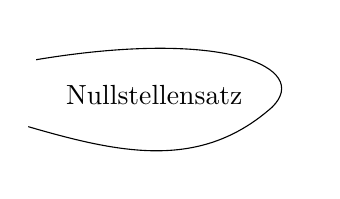
\begin{tikzpicture}
\node at (0,0) {Nullstellensatz};
\draw (-1.5,.45) .. controls (.9,.85) and (2,.35) .. (1.5,-.15) .. controls (.6,-.95) and (-.4,-.75) .. (-1.6,-.4);
\end{tikzpicture}}}

Enfin, pour référence ultérieure, signalons la proposition triviale suivante, (dont nous avons fait déjà usage implicitement):

\uline{Proposition} 1.17. Soient $G\supset H\supset T$ des préschémas en groupes de type fini sur $S$. \deleted{Alors}\inserted{Conditions équivalentes:}

(i) \deleted{Si} $T$ est un tore maximal de $G$, \deleted{c'est un tore maximal de $H$, et \unsure{pour tout $s\in S$ $T_s$ est un tore maximal de $G_s$}}

(ii) \deleted{Si} $T$ est un tore maximal de $H$, et \deleted{si} pour tout $s\in S$, on a égalité des rangs réductifs $\rho_r(G_s)=\rho_r(H_s)$, \deleted{alors $T$ est un tore maximal de $G$}.

2. \uline{Le groupe de Weyl.}

Soit d'abord $k$ un corps algébriquement clos, et soit $G$ un groupe algébrique sur $k$, \inserted{lisse et affine sur $k$.} Si $T$ est un tore maximal, $C$ son centralisateur et $N$ son normalisateur, alors en vertu de \inserted{Exp $\overline{\underline{\mathrm{XI}}}$} 5.9. ce sont des sous-groupes fermés lisses de $G$, \deleted{\unsure{essentiellement}} et $C$ est un sous-groupe ouvert de $N$, de sorte que \inserted{$W=$} $N/C$ est un groupe fini \deleted{\unsure{(et même, qui sera appelé le groupe de Weyl}}\inserted{étale sur $k$, donc déterminé par le groupe $W(k)$} de \deleted{$G$ relativement au tore maximal $T$}. ses points à valeurs dans $k$, comme $W=W(k)_k$ (groupe constant défini par le groupe fini ordinaire $W(k)$). Le groupe fini $W(k)$ s'appelera le \uline{groupe de Weyl géométrique}, (ou simplement groupe de Weyl si une confusion n'est pas à craindre), \uline{de} $G$ \uline{relativement à} $T$. En vertu du théorème de \inserted{conjugaison de} Borel, les groupes de Weyl relatifs aux divers tores maximaux sont isomorphes entre eux, c'est pourquoi on parle parfois ``du'' groupe de Weyl de $G$, sans préciser de tore maximal. \deleted{\unsure{On}} Comme la formation de $C,N$, et $N/C$ commute à toute extension de la base, on voit que si $k'$ est une extension algébriquement close de $k$, le groupe de Weyl géométrique de $G_{k'}$ relativement à $T_{k'}$ est canoniquement \unsure{isomorphe}
\mspage{28}
